% Also note that the "draftcls" or "draftclsnofoot", not "draft", option
% should be used if it is desired that the figures are to be displayed in
% draft mode.
%

\setlength{\paperheight}{11in}
\setlength{\paperwidth}{8.5in}

%\documentclass[conference]{IEEEtran}
%\documentclass{acm_proc_article-sp}
\documentclass{sig-alternate}

% correct bad hyphenation here
\hyphenation{op-tical net-works semi-conduc-tor}

% Optionally save space in lists (place this command after a list environment (e.g., itemize, enumerate, description)
\newcommand{\compresslist}{
	\vspace{-1em}
	\setlength{\itemsep}{1pt}
	\setlength{\parskip}{0pt}
	\setlength{\parsep}{0pt}
}

\usepackage{subfigure}
\usepackage{cite}
\usepackage{url}
\usepackage{tabularx}
\usepackage[table, svgnames]{xcolor} 
\usepackage{color}
\usepackage{siunitx}
\usepackage{multirow}
\usepackage{wasysym}
\usepackage{times}
\usepackage{graphicx}
\usepackage{epsf}
\usepackage{verbatim}
\usepackage{psfig}
\usepackage{cite}
\usepackage{url}
\usepackage{color}
\usepackage[table]{xcolor}
\usepackage{booktabs, dcolumn}
\usepackage{alltt}

\usepackage{longtable,lscape}
\usepackage{slashbox,multirow}
\usepackage{colortbl}
\usepackage{mathrsfs}

\newcommand{\Add}{\CodeIn{add}}
\newcommand{\AVTree}{\CodeIn{AVTree}}
\newcommand{\Assignment}[3]{$\langle$ \Object{#1}, \Object{#2}, \Object{#3} $\rangle$}
\newcommand{\BinaryTreeRemove}{\CodeIn{BinaryTree\_remove}}
\newcommand{\BinaryTree}{\CodeIn{BinaryTree}}
\newcommand{\Caption}{\caption}
\newcommand{\Char}[1]{`#1'}
\newcommand{\CheckRep}{\CodeIn{checkRep}}
\newcommand{\ClassC}{\CodeIn{C}}
\newcommand{\CodeIn}[1]{{\small\texttt{#1}}}
\newcommand{\CodeOutSize}{\scriptsize}
\newcommand{\Comment}[1]{}
\newcommand{\Ensures}{\CodeIn{ensures}}
\newcommand{\ExtractMax}{\CodeIn{extractMax}}
\newcommand{\FAL}{field-ordering}
\newcommand{\FALs}{field-orderings}
\newcommand{\Fact}{observation}
\newcommand{\Get}{\CodeIn{get}}
\newcommand{\HashSet}{\CodeIn{HashSet}}
\newcommand{\HeapArray}{\CodeIn{HeapArray}}
\newcommand{\Intro}[1]{\emph{#1}}
\newcommand{\Invariant}{\CodeIn{invariant}}
\newcommand{\JUC}{\CodeIn{java.\-util.\-Collections}}
\newcommand{\JUS}{\CodeIn{java.\-util.\-Set}}
\newcommand{\JUTM}{\CodeIn{java.\-util.\-TreeMap}}
\newcommand{\JUTS}{\CodeIn{java.\-util.\-TreeSet}}
\newcommand{\JUV}{\CodeIn{java.\-util.\-Vector}}
\newcommand{\JMLPlusJUnit}{JML+JUnit}
\newcommand{\Korat}{Korat}
\newcommand{\Left}{\CodeIn{left}}
\newcommand{\Lookup}{\CodeIn{lookup}}
\newcommand{\MethM}{\CodeIn{m}}
\newcommand{\Node}[1]{\CodeIn{N}$_#1$}
\newcommand{\Null}{\CodeIn{null}}
\newcommand{\Object}[1]{\CodeIn{o}\ensuremath{_#1}}
\newcommand{\PostM}{\MethM$_{post}$}
\newcommand{\PreM}{\MethM$_{pre}$}
\newcommand{\Put}{\CodeIn{put}}
\newcommand{\Remove}{\CodeIn{remove}}
\newcommand{\RepOk}{\CodeIn{repOk}}
\newcommand{\Requires}{\CodeIn{requires}}
\newcommand{\Reverse}{\CodeIn{reverse}}
\newcommand{\Right}{\CodeIn{right}}
\newcommand{\Root}{\CodeIn{root}}
\newcommand{\Set}{\CodeIn{set}}
\newcommand{\State}[1]{2^{#1}}
\newcommand{\TestEra}{TestEra}
\newcommand{\TreeMap}{\CodeIn{TreeMap}}

\newenvironment{CodeOut}{\begin{scriptsize}}{\end{scriptsize}}
\newenvironment{SmallOut}{\begin{small}}{\end{small}}

\newcommand{\pairwiseEquals}{PairwiseEquals}
\newcommand{\monitorEquals}{MonitorEquals}
%\newcommand{\monitorWField}{WholeStateW}
\newcommand{\traverseField}{WholeState}
\newcommand{\monitorSMSeq}{ModifyingSeq}
\newcommand{\monitorSeq}{WholeSeq}

\newcommand{\IntStack}{\CodeIn{IntStack}}
\newcommand{\UBStack}{\CodeIn{UBStack}}
\newcommand{\BSet}{\CodeIn{BSet}}
\newcommand{\BBag}{\CodeIn{BBag}}
\newcommand{\ShoppingCart}{\CodeIn{ShoppingCart}}
\newcommand{\BankAccount}{\CodeIn{BankAccount}}
\newcommand{\BinarySearchTree}{\CodeIn{BinarySearchTree}}
\newcommand{\LinkedList}{\CodeIn{LinkedList}}

\newcommand{\Book}{\CodeIn{Book}}
\newcommand{\Library}{\CodeIn{Library}}

\newcommand{\Jtest}{Jtest}
\newcommand{\JCrasher}{JCrasher}
\newcommand{\Daikon}{Daikon}
\newcommand{\JUnit}{JUnit}

\newcommand{\trie}{trie}

\newcommand{\Perl}{Perl}


\newcommand{\SubjectCount}{11}
\newcommand{\DSSubjectCount}{two}

\newcommand{\Equals}{\CodeIn{equals}}
\newcommand{\Pairwise}{PairwiseEquals}
\newcommand{\Subgraph}{MonitorEquals}
\newcommand{\Concrete}{WholeState}
\newcommand{\ModSeq}{ModifyingSeq}
\newcommand{\Seq}{WholeSeq}
\newcommand{\Aeq}{equality}

\newcommand{\Meaning}[1]{\ensuremath{[\![}#1\ensuremath{]\!]}}
\newcommand{\Pair}[2]{\ensuremath{\langle #1, #2 \rangle}}
\newcommand{\Triple}[3]{\ensuremath{\langle #1, #2, #3 \rangle}}
\newcommand{\SetSuch}[2]{\ensuremath{\{ #1 | #2 \}}}

\newcommand{\Equiv}[2]{\ensuremath{#1 \EquivSTRel{} #2}}
\newcommand{\EquivME}{\Equiv}
\newcommand{\EquivST}{\Equiv}
\newcommand{\EquivSTRel}{\ensuremath{\cong}}
\newcommand{\Redundant}[2]{\ensuremath{#1 \lhd #2}}
\newcommand{\VB}{\ensuremath{\mid}}
\newcommand{\MES}{method-entry state}

\newcommand{\Small}[1]{{\small{#1}}}

\newcommand{\CenterCell}[1]{\multicolumn{1}{c|}{#1}}

% Yoonki's code
\colorlet{tableheadcolor}{gray!25} % Table header colour = 25% gray
\newcommand{\headcol}{\rowcolor{tableheadcolor}} %
\colorlet{tablerowcolor}{gray!10} % Table row separator colour = 10% gray
\newcommand{\rowcol}{\rowcolor{tablerowcolor}} %
    % Command \topline consists of a (slightly modified) \toprule followed by a \heavyrule rule of colour tableheadcolor (hence, 2 separate rules)
\newcommand{\topline}{\arrayrulecolor{black}\specialrule{0.1em}{\abovetopsep}{0pt}%
            \arrayrulecolor{tableheadcolor}\specialrule{\belowrulesep}{0pt}{0pt}%
            \arrayrulecolor{black}}
    % Command \midline consists of 3 rules (top colour tableheadcolor, middle colour black, bottom colour white)
\newcommand{\midline}{\arrayrulecolor{tableheadcolor}\specialrule{\aboverulesep}{0pt}{0pt}%
            \arrayrulecolor{black}\specialrule{\lightrulewidth}{0pt}{0pt}%
            \arrayrulecolor{white}\specialrule{\belowrulesep}{0pt}{0pt}%
            \arrayrulecolor{black}}
    % Command \rowmidlinecw consists of 3 rules (top colour tablerowcolor, middle colour black, bottom colour white)
\newcommand{\rowmidlinecw}{\arrayrulecolor{tablerowcolor}\specialrule{\aboverulesep}{0pt}{0pt}%
            \arrayrulecolor{black}\specialrule{\lightrulewidth}{0pt}{0pt}%
            \arrayrulecolor{white}\specialrule{\belowrulesep}{0pt}{0pt}%
            \arrayrulecolor{black}}
    % Command \rowmidlinewc consists of 3 rules (top colour white, middle colour black, bottom colour tablerowcolor)
\newcommand{\rowmidlinewc}{\arrayrulecolor{white}\specialrule{\aboverulesep}{0pt}{0pt}%
            \arrayrulecolor{black}\specialrule{\lightrulewidth}{0pt}{0pt}%
            \arrayrulecolor{tablerowcolor}\specialrule{\belowrulesep}{0pt}{0pt}%
            \arrayrulecolor{black}}
    % Command \rowmidlinew consists of 1 white rule
\newcommand{\rowmidlinew}{\arrayrulecolor{white}\specialrule{\aboverulesep}{0pt}{0pt}%
            \arrayrulecolor{black}}
    % Command \rowmidlinec consists of 1 tablerowcolor rule
\newcommand{\rowmidlinec}{\arrayrulecolor{tablerowcolor}\specialrule{\aboverulesep}{0pt}{0pt}%
            \arrayrulecolor{black}}
    % Command \bottomline consists of 2 rules (top colour
\newcommand{\bottomline}{\arrayrulecolor{white}\specialrule{\aboverulesep}{0pt}{0pt}%
            \arrayrulecolor{black}\specialrule{\heavyrulewidth}{0pt}{\belowbottomsep}}%
\newcommand{\bottomlinec}{\arrayrulecolor{tablerowcolor}\specialrule{\aboverulesep}{0pt}{0pt}%
            \arrayrulecolor{black}\specialrule{\heavyrulewidth}{0pt}{\belowbottomsep}}%

\usepackage{dcolumn}
\newcolumntype{Y}{D..{6.4}}

%\newcommand{\blind}[1]{{\color{white}\{#1\}}}
\newcommand{\blind}[1]{#1}


%
% paper title
% can use linebreaks \\ within to get better formatting as desired
% Do not put math or special symbols in the title.
\begin{document}
\title{Questions Developers Ask While Diagnosing Potential Security Vulnerabilities With Static Analysis}
% What Questions Do Developers Ask When Reasoning about the Security of Their Code? Building Tools that Answer Developers' Questions about Security Vulnerabilities?

\numberofauthors{2}
\author{
\alignauthor Justin Smith, Brittany Johnson, and Emerson Murphy-Hill\\
\affaddr{North Carolina State University}\\
\affaddr{Raleigh, NC 27606} \\
\email{\{jssmit11, bijohnson\}@ncsu.edu, emerson@csc.ncsu.edu}
\alignauthor Bill Chu and Heather Richter Lipford\\
\affaddr{University of North Carolina at Charlotte}\\
\affaddr{Charlotte, NC 28223}\\
\email{\{billchu, heather.lipford\}@uncc.edu}
%\blind{\{billchu, heather.lipford\}@uncc.edu}
}

\maketitle


% As a general rule, do not put math, special symbols or citations
% in the abstract
\begin{abstract}

Security tools can help developers answer questions about potential vulnerabilities in their code. 
A better understanding of the types of questions asked by developers may help toolsmiths design more effective tools.
In this paper, we describe how we collected and categorized these questions 
by conducting an exploratory study with novice and experienced software developers.
We equipped them with Find Security Bugs, a security-oriented static analysis tool, and observed their interactions with security vulnerabilities in an open-source system that they had previously contributed to.
We found that they asked questions not only about security vulnerabilities, associated attacks, and fixes,
but also questions about the software itself, the social ecosystem that built the software,
and related resources and tools.
For example, when participants asked questions about the source of tainted data,
their tools forced them to make imperfect tradeoffs between 
systematic and ad hoc program navigation strategies.
%Our results have several implications for designing security tools that support developers
%by helping them answer their questions.
\end{abstract}
% no keywords


\section{Introduction}

%Security is critical
Software developers are a critical part of making software secure, a particularly important task considering security vulnerabilities are likely to cause incidents that affect company profits as well as end users~\cite{chen2002mops}.
When software systems contain security defects, developers are responsible for fixing them. 

%Tools help developers with security
To assist developers with the task of detecting and removing security defects, toolsmiths provide a variety of static analysis tools.
One example of such a tool is Find Security Bugs (FSB)~\cite{FindSecurityBugs}, an extension of FindBugs~\cite{FindBugs}.
FSB locates and reports on potential software security vulnerabilities, such as SQL injection and cross-site scripting.  
Other tools, such as CodeSonar~\cite{CodeSonar} and Coverity~\cite{Coverity}, can also be used to detect and remove potential security vulnerabilities.
In fact, toolsmiths have created over 50, both free and commercial, static analysis tools to help developers secure their systems~\cite{CodeAnalysis, OWASPSCA, SecurityAnalyzers}.

These tools provide, for instance, information about the locations of potential SQL injection vulnerabilities.
%But developers don't use them because they don't provide right information
Unfortunately, despite their availability, research suggests that developers do not use static analysis tools, partially because the tools provide information that does not adequately align with their information needs~\cite{johnson2013don}. 

Our work addresses this problem by advancing our understanding of developers' information needs while interacting with a security-focused static analysis tool. 
To our knowledge, no prior study has specifically investigated developers' information needs while using such a tool. 
As we show later in this paper, developers need unique types of information while assessing security vulnerabilities, like information about attacks.

%And this work has improved the effectivness of tools
In non-security domains, similar work that identifies information needs has helped toolsmiths both evaluate the effectiveness of existing tools~\cite{ammar2012empirical}, and improve the state of program analysis tools~\cite{kononenko2012automatically, servant2012history, yoon2013visualization}. 
Similarly, we expect that categorizing developers' information needs while using security-focused static analysis tools will help researchers evaluate and toolsmiths improve those tools. 

%What we did
To that end, we conducted a exploratory study with ten developers who had contributed to iTrust~\cite{iTrust}, a security-critical Java medical records software system.
We observed each developer as they assessed potential security vulnerabilities identified by FSB. 
We operationalized developers' information needs by measuring questions --- the verbal manifestations of information needs. 
We report the questions participants asked throughout our study and discuss the strategies participants used to answer their questions.
Using a card sort methodology, we sorted 559 questions into 17 categories. 
The primary contribution of this work is a categorization of questions, which researchers and toolsmiths can use to inform the design of more usable static analysis tools.

%Figure, high res, png or vector (pdf)

\section{Related Work}
\label{sec:rw}

We have organized the related work into two subsections. 
Section \ref{evaluation} outlines some of the current approaches researchers use to evaluate security tools and Section \ref{questions} references other studies that have explored developers' information needs.

\subsection{Evaluating Security Tools}
\label{evaluation}
Using a variety of metrics, many studies have assessed the effectiveness of the security tools developers use to find and remove vulnerabilities from their code~\cite{martin2005finding, austin2011one, livshits2005finding}.  

Much research has evaluated the effectiveness of tools based on their false positive rates and how many vulnerabilities they detect~\cite{jovanovic2006pixy, austin2011one, dukes2013case}. 
For instance, Jovanovic and colleagues evaluate their tool, \textsc{Pixy}, a static analysis tool that detects cross-site scripting vulnerabilities in PHP web applications~\cite{jovanovic2006pixy}. 
They considered \textsc{Pixy} effective because of its low false positive rate (50\%) and its ability to find vulnerabilities previously unknown. 
Similarly, Livshits and Lam evaluated their own approach to security-oriented static analysis, which creates static analyzers based on inputs from the user~\cite{livshits2005finding}. 
They also found their tool to be effective because it had a low false positive rate. 

Austin and Williams compared the effectiveness of four existing techniques for discovering security vulnerabilities: systematic and exploratory manual  penetration testing, static analysis, and automated penetration testing~\cite{austin2011one}. 
Comparing the four approaches based on number of vulnerabilities found, false positive rate, and efficiency, they reported that no one technique was capable of discovering every type of vulnerability. 

Dukes and colleagues conducted a case study comparing static analysis and manual testing techniques used to find security vulnerabilities~\cite{dukes2013case}. 
They found combining manual testing and static analysis was most effective, because it located the most vulnerabilities.

These studies use various measures of effectiveness, such as false positive rates or vulnerabilities found by a tool, but none focus on how developers interact with the tool. 
Further, these studies do not evaluate whether the tools address developers' information needs. 
Unlike existing studies, our study focuses on developers' information needs while assessing security vulnerabilities and, accordingly, provides a novel framework for evaluating security tools.

\subsection{Information Needs Studies}
\label{questions}
Several studies have explored the developers' information needs outside the context of security.
Similar to our work, some existing studies determine these needs by focusing on the questions developers ask~\cite{latoza2010hard, latoza2010developers}.
In contrast, our study focuses specifically on the information needs of developers while assessing security vulnerabilities.


Much of the work on answering developer questions has occurred in the last decade. 
LaToza and Myers surveyed professional software developers to understand the questions developers ask during their daily coding activities, focusing on the hard to answer questions~\cite{latoza2010hard}. 
Furthermore, after observing developers in a lab study, they discovered that the questions developers ask tend to be questions revolving around searching through the code for target statements or reachability questions~\cite{latoza2010developers}. 
Ko and Myers developed \textsc{Whyline}, a tool meant to ease the process of debugging code by helping answer ``why did'' and ``why didn't'' questions~\cite{ko2004designing}. 
They found that developers were able to complete more debugging tasks while using their tool than they could without it.
Fritz and Murphy developed a model and prototype tool to assist developers with answering the questions they want to ask based on interviews they conducted~\cite{fritz2010using}.


\section{Methodology}
\label{sec:meth}
We conducted an exploratory study with ten software developers. In our analysis, we extracted and categorized the questions developers asked during each study session. 
Section \ref{rqs} outlines the research question we sought to answer. 
Section \ref{studyDesign} details how the study was designed and Section \ref{dataAnalysis} describes how we performed data analysis.
Study materials can be found online~\cite{ExperimentalMaterials}.

\subsection{Research Question}
\label{rqs}
We want to answer the following research question: What information do developers need while using static analysis tools to diagnose potential security vulnerabilities? 
We measured developers' information needs by examining the questions they asked.
The questions that we identified are all available online~\cite{ExperimentalMaterials} and several exemplary questions are listed in the results sections.
Where possible, we also link questions to the tools and strategies that developers used to answer their questions.


\subsection{Study Design}
\label{studyDesign}
To ensure all participants were familiar with the study environment and Find Security Bugs (FSB),
each in-person session started with a five-minute briefing section, which included a demonstration of FSB and time for questions.
During the briefing section, we asked participants to act as if they were in charge of security for iTrust.
Additionally, we asked them to use a think-aloud protocol, which encourages  participants to verbalize their thought process as they complete a task or activity~\cite{nielsen2002getting}. 
Specifically, they were asked to: ``Say any questions or thoughts that cross your mind regardless of how relevant you think they are.''
We recorded both audio and the screen as study artifacts for data analysis.

Following the briefing period, participants progressed through encounters with four vulnerabilities. 
Figure \ref{fig:environment} depicts the configuration of the integrated development environment (IDE) for one of these encounters.
All participants consented to participate in our study, which had institutional review board approval, and to have their session recorded using screen and audio capture software.
Finally, each session concluded with several demographic and open-ended discussion questions.

\begin{figure}
	\subfigcapskip = 5pt
	\subfigure[Navigation]{
		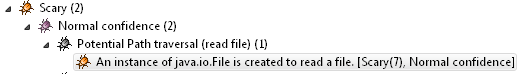
\includegraphics[width=\columnwidth]{Images/Nav.png}
	}
	
	\subfigcapskip = 5pt
	\subfigure[Code]{
	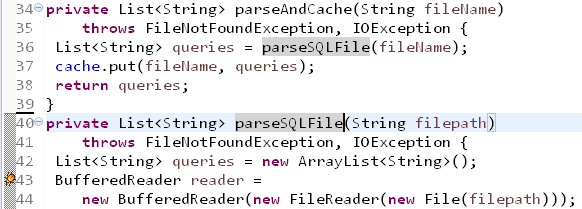
\includegraphics[width=\columnwidth]{Images/Code.png}
	}
	
	\subfigcapskip = 5pt
	\subfigure[Short Notification Text]{
		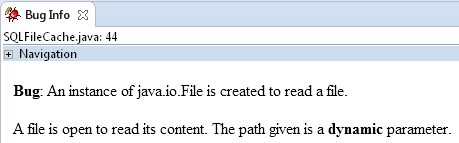
\includegraphics[width=\columnwidth]{Images/BugInfo.png}
	}
	

	\caption{The study environment.}
	\label{fig:environment} 
\end{figure}



\subsubsection{Materials}
Participants used Eclipse to explore vulnerabilities in iTrust, an open source Java medical records web application that ensures the privacy and security of patient records according to the HIPAA statute~\cite{HIPAA}. 
Participants were equipped with FSB, an extended version of FindBugs.

We chose FSB because it detects security defects and compares to other program analysis tools, such as those listed by NIST,~\cite{SecurityAnalyzers} OWASP,~\cite{OWASPSCA} and WASC~\cite{CodeAnalysis}. 
Some of the listed tools may include more or less advanced bug detection features. 
However, FSB is representative of static analysis security tools with respect to its user interface, specifically in how it communicates with its users.
FSB provides visual code annotations and textual notifications that contain vulnerability-specific information.
It summarizes all the vulnerabilities it detects in a project and allows users to prioritize potential vulnerabilities based on several metrics such as bug type or severity.


\begin{table}
\centering
\caption{Demographics of study participants}
\begin{tabular}{|l|l|c|S|}
\rowcolor{gray!50}
\hline
    Participant		& Job Title 						& Vulnerability 			&\multicolumn{1}{c|}{Experience} \\
    \rowcolor{gray!50}
    				&									& Familiarity				&   \multicolumn{1}{c|}{Years} \\
    \hline
    P1			    & Student     						& \CIRCLE{}\CIRCLE{}\LEFTcircle{}\Circle{}\Circle{} 	&  4.5    \\
    \hline
    P2			    & Test Engineer    					& \CIRCLE{}\CIRCLE{}\CIRCLE{}\Circle{}\Circle{}		&  8 		\\
    \hline
    P3 				& Development Tester       			& \CIRCLE{}\CIRCLE{}\Circle{}\Circle{}\Circle{}		&  6 	    	\\
    \hline
    P4				& Software Developer     			& \CIRCLE{}\CIRCLE{}\Circle{}\Circle{}\Circle{}			&  6     	\\
    \hline
    P5				& Student      						& \CIRCLE{}\CIRCLE{}\CIRCLE{}\CIRCLE{}\Circle{}			&  10 	\\
    \hline
    P6				& Student		    				& \CIRCLE{}\Circle{}\Circle{}\Circle{}\Circle{}			& 4		\\
    \hline
    P7				& Software Developer    	& \CIRCLE{}\CIRCLE{}\CIRCLE{}\CIRCLE{}\Circle{}		& 4.5         \\
    \hline
    P8				& Student	    					& \CIRCLE{}\CIRCLE{}\CIRCLE{}\Circle{}\Circle{}		& 7   \\
    \hline
    P9				& Software Consultant   	 		& \CIRCLE{}\CIRCLE{}\CIRCLE{}\Circle{}\Circle{}		& 5	  		 \\
    \hline
    P10			    & Student    						& \CIRCLE{}\CIRCLE{}\CIRCLE{}\Circle{}\Circle{}		& 8	           \\
    \hline
\end{tabular}
\label{table:participants}
\end{table}



\subsubsection{Participants}
For our study, we recruited ten software developers, five students and five professionals. 
Table~\ref{table:participants} gives additional demographic information on each of the ten participants. 
Participants ranged in programming experience from 4 to 10 years, averaging 6.3 years.
Participants also self-reported their familiarity with security vulnerabilities on a 5 point Likert scale, with a median of 3.
Although we report on experiential and demographic information, the focus of this work is to identify questions that span experience levels.
In the remainder of this paper, we will refer to participants by the abbreviations found in the participant column of the table.

We faced the potential confound of measuring participants questions about a new code base rather than measuring their questions about vulnerabilities.
To mitigate this confound, we required participants to be familiar with iTrust;
all participants either served as teaching assistants for, or completed a semester-long software engineering course that focused on developing iTrust.
This requirement also ensured that participants had experience using static analysis tools similar to FSB.

However, this requirement restricted the size of our potential participant population.
Accordingly, we used a nonprobabilistic, purposive sampling approach~\cite{guest2006many}, which typically yields fewer participants, but gives deeper insights into the observed phenomena.
To identify eligible participants, we recruited via personal contacts, class rosters, and asked participants at the end of the study to recommend other qualified participants.
Although our study involved only ten participants, we reached saturation~\cite{glaser2009discovery} rather quickly; 
no new question categories were introduced after the fourth participant.
%ideographic, nomethethic, or typical size, grounded theory
%Typical grounded theory analysis involves X, Y, Z. Other work has reached saturation at X Participants. 

%

%This format has fewer participants but gives deeper insight.

%Since extracting data from each session required intensive analysis, we ceased recruitment when we determined that we had reached saturation~\cite{glaser2009discovery} and few new questions were emerging from each additional session.

  
\subsubsection{Tasks}
First we conducted a preliminary pilot study ($n = 4$), in which  participants spent approximately 10 to 15 minutes with each task and showed signs of fatigue after 60 minutes.
To reduce the effects of fatigue, we asked each participant to assess four vulnerabilities. 
We do not report on data collected from this preliminary study.

When selecting tasks, we ran FSB on iTrust and identified 118 potential security vulnerabilities, across three topics.
To increase the diversity of responses, we selected tasks from mutually exclusive topics, as categorized by FSB.
For the fourth task, we added a SQL injection vulnerability to iTrust by making minimal alterations to one of the database access objects.
Our alterations preserved the functionality of the original code and were based on examples of SQL injection found on OWASP~\cite{OWASP} and in open-source projects.
We chose to add a SQL injection vulnerability, because among all security vulnerabilities, OWASP ranks injection vulnerabilities as the most critical web application security risk.
Table \ref{table:vulnerabilities} summarizes each of the four tasks. 

\begin{table*} 
\centering
\caption{Four vulnerability exploration tasks}
\begin{tabularx}{\textwidth}{|l|X|l|}
\rowcolor{gray!50}
\hline
    Vulnerability				& Short Description													& Severity Rank 	\\
    \hline	
    Potential Path Traversal	& An instance of java.io.File is created to read a file.     			& ``Scary''	    \\
    \hline
    Predictable Random			& Use of java.util.Random is predictable. 								& ``Scary''		\\
    \hline
    Servlet Parameter 			& The method getParameter returns a String value that is controlled by the client.			& ``Troubling''	\\
    \hline
    SQL Injection				& [Method name] passes a non-constant String to an execute method on an SQL statement.     	& ``Of Concern'' \\
    \hline
\end{tabularx}
\label{table:vulnerabilities}
\end{table*}


\subsection{Data Analysis}
\label{dataAnalysis}
To analyze the data, we first transcribed all the audio-video files using oTranscribe~\cite{OTranscribe}.
Each transcript, along with the associated recording, was analyzed by two of the authors for implicit and explicit questions. 
The two question sets for each session were then iteratively compared against each other until the authors reached agreement on the question sets. 
In the remainder of this section, we will detail the question extraction process and question sorting processes, including the criteria used to determine which statements qualified as questions.
\subsubsection{Question Criteria}
Participants ask both explicit and implicit questions. 
Drawing from previous work on utterance interpretation~\cite{letovsky1987cognitive}, we developed five criteria to assist in the uniform classification of participant statements. 
A statement was coded as a question only if it met one of the following criteria:
\\
\begin{itemize}
\compresslist	
\item \textbf{The participant explicitly asks a question.}
\\ Example: \textit{Why aren't they using \CodeIn{PreparedStatements}?}
\item \textbf{The participant makes a statement and explores the validity of that statement.}
\\ Example: \textit{It doesn't seem to have shown what I was looking for. Oh, wait! It's right above it...}
\item \textbf{The participant uses key words such as, ``I assume,'' ``I guess,'' or ``I don't know.''}
\\ Example: \textit{I don't know that it's a problem yet.}
\item \textbf{The participant clearly expresses uncertainty over a statement.}
\\ Example: \textit{Well, it's private to this object, right?}
\item \textbf{The participant clearly expresses an information need by describing plans to acquire information.}
\\ Example: \textit{I would figure out where it is being called.}

\end{itemize}

\begin{figure*}
	\centering
	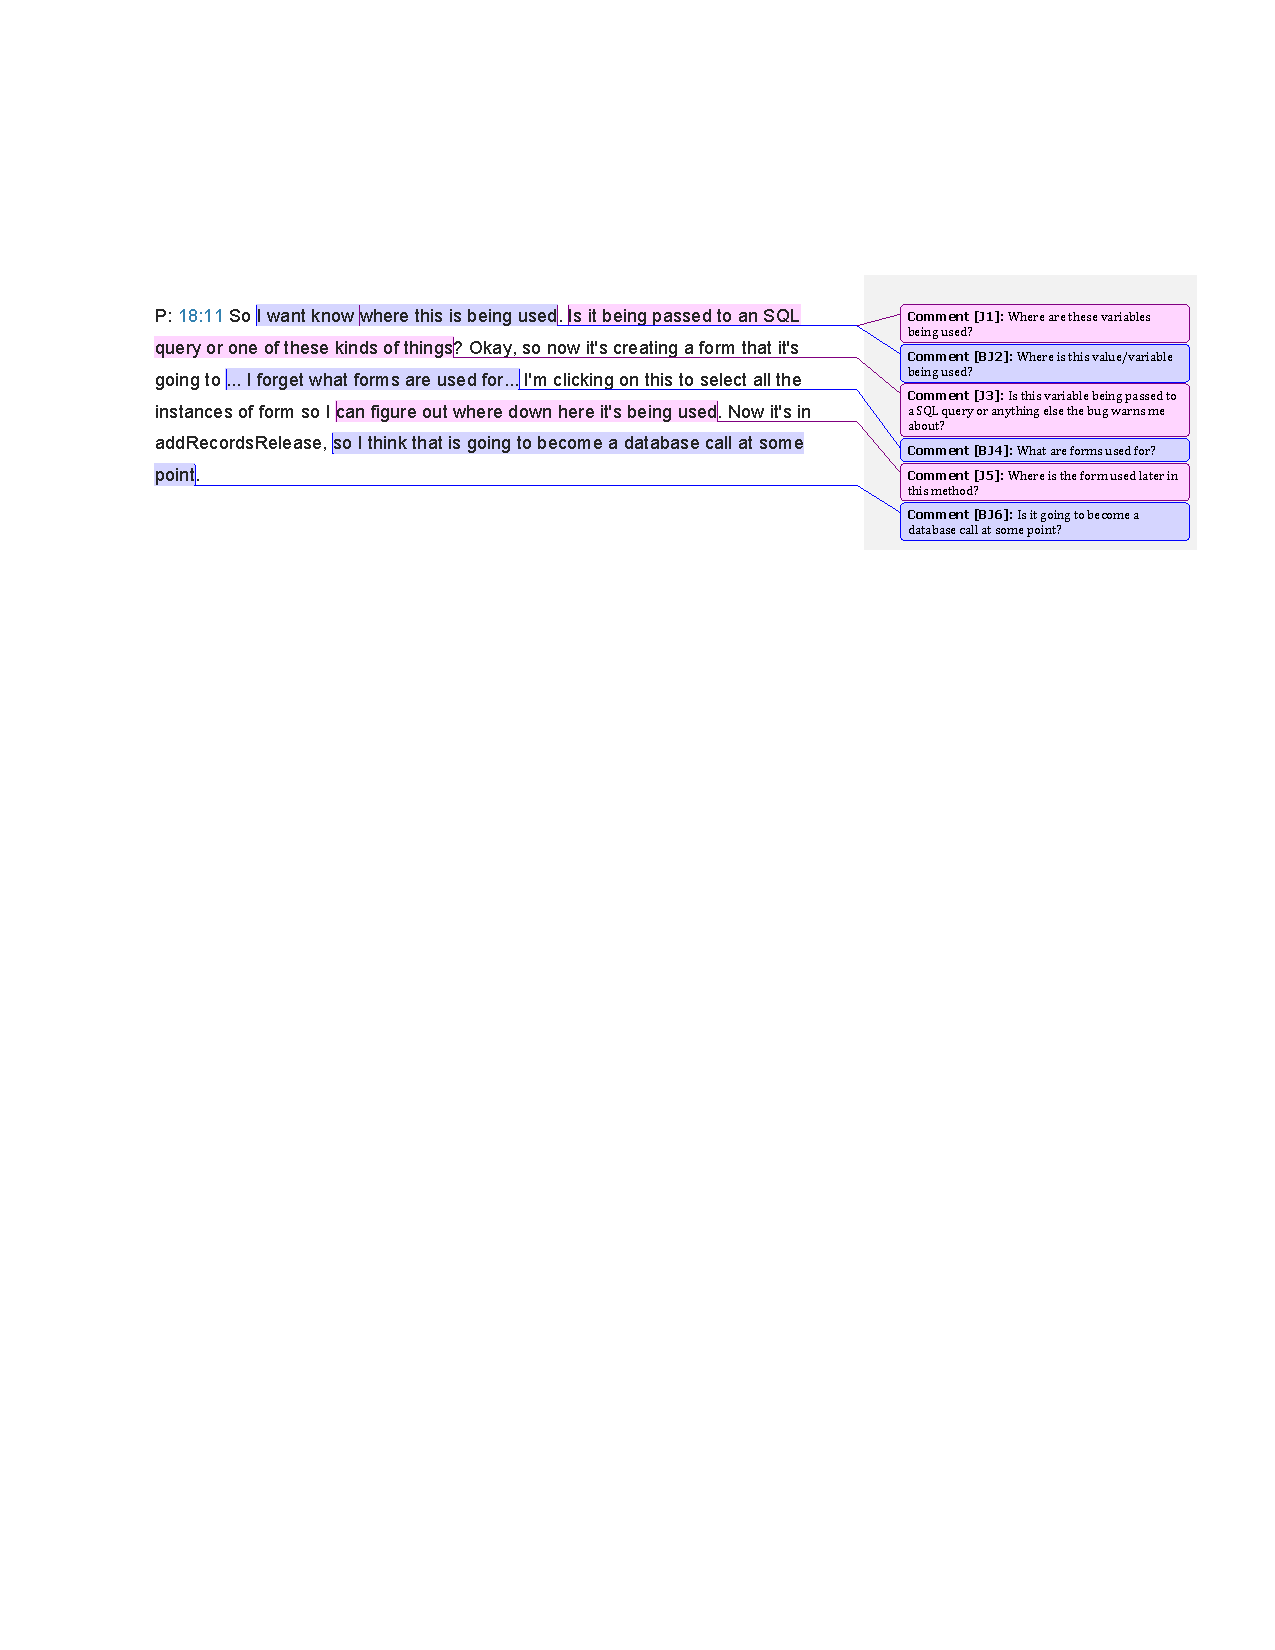
\includegraphics[width=7.5in]{Images/QuestionMerging}
	\caption{Question merging process}
	\label{fig:merging} 
\end{figure*}


\subsubsection{Question Extraction}
To make sure our extraction was exhaustive, the first two authors independently coded each transcript using the criteria outlined in the previous section.
When we identified a statement that satisfied one or more of the above criteria, we marked the transcript, highlighted the participant's original statement, and clarified the question being asked.
Question clarification typically entailed rewording the question to best reflect the information the participant was trying to acquire.
From the ten sessions, the first coder extracted 421 question statements; the other coder extracted 389. 

It was sometimes difficult to determine what statements should be extracted as questions; the criteria helped ensure both authors only highlighted the statements that reflected actual questions. 
Figure \ref{fig:merging} depicts a section of the questions extracted by both authors from P8 prior to review.


\subsubsection{Question Review}
To remove duplicates and ensure the validity of all the questions, each transcript was reviewed jointly by the two authors who initially coded it.
During this second pass, the two reviewers examined each question statement, discussing the justification for each question based on the previously stated criteria.
The two reviewers merged duplicate questions, favoring the wording that was most strongly grounded in the study artifacts.
This process resulted in a total of 559 questions.

Each question that was only identified by one author required verification.
If the other author did not agree that such a question met at least one of the criteria, the question was removed from the question set and counted as a disagreement.
The reviewers were said to agree when they merged a duplicate or verified a question. Depending on the participant, inter-reviewer agreement ranged from 91\% to 100\%. Across all participants, agreement averaged to 95\%.
The agreement scores suggest that the two reviewers consistently held similar interpretations of the question criteria.

It is also important to note that participants' questions related to several topics in addition to security. 
We discuss the questions that are most closely connected to security in Sections \ref{pupa}, \ref{eui}, and \ref{bsr}.
Although our primary focus is security, we are also interested in the other questions that participants posed, as those questions often have security implications.
For example, researchers have observed that developers ask questions about data flow, like \emph{What is the original source of this data}, even outside security~\cite{latoza2010hard}.
However, in a security context, this question is particularly important, because potentially insecure data sources often require special handling to prevent attacks.


\subsubsection{Question Sorting}
To organize our questions and facilitate discussion, we performed an \textit{open} card sort~\cite{hudson2013sorting}. 
Card sorting is typically used to help structure data by grouping related information into categories. 
In an \textit{open} sort, the sorting process begins with no notion of predefined categories. 
Rather, sorters derive categories from emergent themes in the cards. 

We performed our card sort in three distinct stages: clustering, categorization, and validation.
In the first stage, we formed question clusters by grouping questions that identified the same information needs. 
In this phase we focused on rephrasing similar questions and grouping duplicates.
For example, P1 asked, \textit{Where can I find information related to this vulnerability?} P7 asked, \textit{Where can I find an example of using \CodeIn{PreparedStatements}?} and P2 asked, \textit{Where can I get more information on path traversal?} 
Of these questions, we created a question cluster labeled \textit{Where can I get more information?}
At this stage, we discarded five unclear or non pertinent questions and organized the remaining 554 into 155 unique question clusters.


\begin{table*} 
\centering
\caption{Organizational Groups and Emergent Categories}
\begin{tabularx}{\textwidth}{|l|X|r|c|}
\rowcolor{gray!50}
\hline
    Group											& Category										& Clusters		& Location in Paper	  	\\
    \hline			
    \multirow{4}{*}{Vulnerabilities, Attacks, and Fixes}
        											& Preventing and Understanding Potential Attacks	& 11     		& Section~\ref{pupa}		\\
        											
        											& Understanding Alternative Fixes and Approaches	& 11     		& Section~\ref{uafa}	\\

    												& Assessing the Application of the Fix				& 9     		& Section~\ref{aaf}				\\

    												& Relationship Between Vulnerabilities							& 3     		& Section~\ref{rbb}			\\
    \hline
    \multirow{4}{*}{Code and the Application}	
    												& Locating Information 								& 11      		& Section~\ref{li}		\\

    												& Control Flow and Call Information					& 13     		& Section~\ref{cf}	\\

    												& Data Storage and Flow								& 11     		& Section~\ref{dsf}  	\\

    												& Code Background and Functionality	 				& 17     		& Section~\ref{cbf}			\\

    									& Application Context/Usage										& 9     		& Section~\ref{acu}			\\

    									& End-User Interaction											& 3     		& Section~\ref{eui}		\\
    \hline	
    \multirow{4}{*}{Individuals}	
    									& Developer Planning and Self-Reflection						& 14    		& Section~\ref{dpr}		\\

    									& Understanding Concepts										& 6 			& Section~\ref{uc}			\\

    									& Confirming Expectations					 					& 1				& Section~\ref{ce}  \\
    \hline
	\multirow{4}{*}{Problem Solving Support}

   	 									& Resources and Documentation									& 10     		& Section~\ref{rd}		\\
   	 									
 
    									
    									& Understanding and Interacting with Tools						& 9     		& Section~\ref{uit}			\\

										& Vulnerability Severity and Rank								& 4     		& Section~\ref{bsr}		\\
 
    									& Notification Text												& 3     		& Section~\ref{em}		\\
  
    \hline	
       									& Uncategorized													& 10    		&			 \\
    \hline
\end{tabularx}
\label{table:categories}
\end{table*}


In the second stage, we identified emergent themes and grouped the clusters into categories based on the themes. 
For example, we placed the question \textit{Where can I get more information?} into a category called \emph{\textbf{Resources/Documentation}}, along with questions like \textit{Is this a reliable/trusted resource?} and \textit{What information is in the documentation?} 
Table~\ref{table:categories} contains the 17 categories along with the number of distinct clusters each contains. 

To validate the categories that we identified, we asked two independent researchers to sort the question clusters into our categories. 
Rather than sort the entire set of questions, we randomly selected 43 questions for each researcher to sort.
The first agreed with our categorization with a Cohen's Kappa of $\kappa = .63$. 
Between the first and second researcher we reworded and clarified some ambiguous questions. The second researcher exhibited greater agreement ($\kappa = .70$). 
These values are within the $.60 - .80$ range, indicating substantial agreement~\cite{Landis1977agreement}.

\section{Results}

\subsection{Interpreting the Results}
\label{sec:results}

In the next four sections, we discuss our study's results using the categories we described in the previous section.
Due to their large number, we grouped the categories to organize and facilitate discussion about our findings. 
Table~\ref{table:categories} provides an overview of these groupings.

For each category, we selected several questions to discuss. A full categorization of questions can be found online~\cite{ExperimentalMaterials}.
The numbers next to the category titles denote the number of participants that asked questions in that category and the total number of questions in that category --- in parenthesis and brackets respectively. Similarly, the number in parenthesis next to each question marks the number of participants that asked that question.

The structure of most results categories consists of three parts: an overview of the category, several of the questions we selected, and a discussion of those questions.
However, some sections do not contain any discussion either because participants' intentions in asking those questions were unclear, or participants asked the questions without following up or attempting to answer them at all. 

When discussing the questions participants asked for each category, we will use phrases such as ``\emph{X} participants asked \emph{Y}.''
Note that this work is exploratory and qualitative in nature.
Though we present information about the number of participants who ask specific questions, the reader should not infer any quantitative generalizations.

\subsection{Vulnerabilities, Attacks, and Fixes}
\label{sec:results-vaf}
% next paragraph, go into description of first group 


%%%%%%%%%%%% Preventing and Understanding Potential Attacks 

\subsubsection{\textbf{Preventing and Understanding Potential Attacks (10)\{11\}}}\label{pupa}
Unlike other types of code defects that may cause code to function unexpectedly or incorrectly, security vulnerabilities expose the code to potential attacks. For example, the Servlet Parameter vulnerability (Table~\ref{table:vulnerabilities}) introduced the possibility of SQL injection, path traversal, command injection, and cross-site scripting attacks.
\\

\noindent\emph{Is this a real vulnerability? (7)} \\
\emph{What are the possible attacks that could occur? (5)} \\
\emph{Why is this a vulnerability? (3)} \\
\emph{How can I prevent this attack? (3)} \\
\emph{How can I replicate an attack to exploit this vulnerability? (2)} \\
\emph{What is the problem (potential attack)? (2)} 
\\

Participants sought information about the types of attacks that could occur in a given context.
To that end, five participants asked, \textit{What are the possible attacks that could occur?}
For example, within the first minute of his analysis P2 read the notification about the Path Traversal vulnerability and stated, ``I guess I'm thinking about different types of attacks.''
Before reasoning about how a specific attack could be executed, he wanted to determine which attacks were relevant to the notification.

Participants also sought information about specific attacks from the notification, asking how particular attacks could exploit a given vulnerability.
Participants hypothesized about specific attack vectors, how to execute those attacks, and how to prevent those attacks now and in the future.
Seven participants, concerned about false positives, asked the question, \textit{Is this a real vulnerability?} 
To answer that question, participants searched for hints that an attacker could successfully execute a given attack in a specific context. 
For example, P10 determined that the Predictable Random vulnerability was ``real'' because an attacker could deduce the random seed and use that information to determine other users' passwords. 


%Some Find Security Bugs notifications attempt to provide developers with the means to answer some of these questions by providing links to relevant information. 
%Many of the links provided linked to information regarding why the code may be broken, however, do not provide information to improve understanding of what the potential attacks are. 
%Some of the questions, such as \textit{How do I find out if this is a real vulnerability?}, may not be as simple to answer by providing a link. 
%This kind of question may require triangulation of information; some information from the web on the vulnerability itself and the potential attacks, and some information from fellow developers who may better understand the likelihood the bug is a vulnerability in their system. 
%One way tools can help is by providing easy access to the top web resources and developers to use when assessing the vulnerability; many of our participants preferred StackOverflow as a resource and a degree of knowledge model, like the one proposed by Fritz and his colleagues, could provide the developers most familiar with the code~\cite{fritz2010degree}.

%%%%%%%%%%%% Understanding Alt. Fixes

\subsubsection{\textbf{Understanding Alternative Fixes and Approaches (8)\{11\}}}\label{uafa}

When resolving security vulnerabilities, participants explored alternative ways to achieve the same functionality more securely.
For example, while evaluating the SQL Injection vulnerability, participants found resources that suggested using the \CodeIn{PreparedStatement} Class instead of Java \CodeIn{Statement} Class. 
\\

\noindent\emph{Does the alternative function the same as what I'm currently using? (6)} \\
\emph{What are the alternatives for fixing this? (4)} \\
\emph{Are there other considerations to make when using the alternative(s)? (3)} \\
\emph{How does my code compare to the alternative code in the example I found? (2)} \\
\emph{Why should I use this alternative method/approach to fix the vulnerability? (2)} 
\\
 
%The developer could attempt to apply the new fix or approach, but the data we report in Section~\ref{aaf} suggests developers also have questions about this process that make it difficult to quickly and effectively complete.
%SAVE THIS CONNECTION FOR LATER
Some notifications, including those for the SQL Injection and Predictable Random vulnerabilities, explicitly offered alternative fixes. 
In other cases, participants turned to a variety of sources, such as StackOverflow, official documentation, and personal blogs for alternative approaches.
 
Three participants specifically mentioned StackOverflow as a source for better understanding alternative approaches and fixes. 
P7 preferred StackOverflow as a resource, because it included real-world examples of broken code and elaborated on why the example was broken.
Despite the useful information some participants found, often the candidate alternative did not readily provide meta-information about the process of applying it to the code. 
For example, P9 found a suggestion on StackOverflow that he thought might work, but it was not clear if it could be applied to the code in iTrust.

While attempting to assess the Servlet Parameter vulnerability, P8 decided to explore some resources on the web and came across a resource that appeared to be affiliated with OWASP~\cite{OWASP}. 
Because he recognized OWASP as ``the authority on security,'' he clicked the link and used it to make his final decision regarding the vulnerability. 
It seemed important to P8 that recommended approaches came from trustworthy sources.

%One way a tool might help developers determine the changes, if any, they should making would be by noting other places in the code the alternative under  consideration has been used, if they exist. 

%The tool could then potentially use speculative analysis, which is used by tools like \textsc{Quick Fix Scout}, to present trade-offs of using the suggested fix or keeping the code as it is~\cite{mucslu2012speculative}.

%GOOD POINTS ABOVE NOT SURE HOW THEY FIT WITH STORY


%If the developer, or other developers of the code, have not used the alternative before, the tool could borrow behavior or design principles from \textsc{Whyline} by allowing developers to ask questions about the code in relation to the suggested approach~\cite{ko2004designing}. 






%%%%%%%%%%%% Assessing Application % % % % % % % % % % % % % % % % % % % % % % % %

\subsubsection{\textbf{Assessing the Application of the Fix (9)\{9\}}}\label{aaf}
Once participants had identified an approach for fixing a security vulnerability (Section \ref{uafa}), they asked questions about applying the fix to the code.
For example, while considering the use of \CodeIn{SecureRandom} to resolve the Predictable Random vulnerability, participants questioned the applicability of the fix and the consequences of making the change. 
The questions in this category differ from those in \emph{\textbf{Understanding Alternative Fixes and Approaches}} (Section \ref{uafa}). 
These questions focus on the process of applying  and reasoning about a given fix, rather than identifying and understanding possible fixes.
\\

\noindent\emph{Will the notification go away when I apply this fix? (5)} \\
\emph{How do I use this fix in my code? (4)} \\
\emph{How do I fix this vulnerability? (4)} \\
\emph{How hard is it to apply a fix to this code? (3)} \\
\emph{Is there a quick fix for automatically applying a fix? (2)} \\
\emph{Will the code work the same after I apply the fix? (2)} \\
\emph{What other changes do I need to make to apply this fix? (2)} 
\\

 
When searching for approaches to resolve vulnerabilities, participants gravitated toward fix suggestions provided by the notification.
As noted above, the notifications associated with the Predictable Random vulnerability and the SQL Injection vulnerability both provided fix suggestions.
All participants proposed solutions that involved applying one or both of these suggestions. 
Specifically, P2 commented that it would be nice if all the notifications contained fix suggestions.

However, unless prompted, none of the participants commented on the disadvantages of using fix suggestions.
While exploring the Predictable Random vulnerability, many participants, including P1, P2, and P6, decided to use \CodeIn{SecureRandom} without considering any alternative solutions, even though the use of that suggested fix reduces performance.
It seems that providing suggestions without discussing the associated trade-offs appeared to reduce participants' willingness to think broadly about other possible solutions. 


%%%%%%%%%%%% Relationship Between Vulnerabilities

\subsubsection{\textbf{Relationship Between Vulnerabilities (4)\{3\}}}\label{rbb}

Some participants asked questions about the connections between co-occurring vulnerabilities and whether similar vulnerabilities exist elsewhere in the code. 
For example, when participants reached the third and fourth vulnerabilities, they began speculating about the similarities between the vulnerabilities they inspected.
\\

\noindent\emph{Are all the vulnerabilities related in my code? (3)} \\
\emph{Does this other piece code have the same vulnerability as the code I'm working with? (1)} 
\\


\subsection{Code and the Application}
\label{sec:results-ca}

% description of what categories fall into this group

%%%%%%%%%%%% Locating Information

\subsubsection{\textbf{Locating Information (10)\{11\}}}\label{li}

Participants asked questions about locating information in their coding environments.
In the process of investigating vulnerabilities, participants searched for information across multiple classes and files.
Unlike Sections \ref{cf} and \ref{dsf}, questions in this category more generally refer to the process of locating information, not just about locating calling information or data flow information.
\\

\noindent\emph{Where is this used in the code? (10)} \\
\emph{Where are other similar pieces of code? (4)} \\
\emph{Where is this method defined? (1)} 
\\

All ten participants wanted to locate where defective code and tainted values were in the system. 
Most of these questions occurred in the context of assessing the Predictable Random vulnerability.
Specifically, participants wondered where the potentially insecure random number generator was being used and whether it was employed generate sensitive data like passwords.

%Where is similar code?
In other cases, while fixing one method, four participants wanted to find other methods that implemented similar functionality.
They hypothesized that other code modules implemented the same functionality using more secure patterns. 
For example, while assessing the SQL Injection vulnerability, P2 and P5 both wanted to find other modules that created SQL statements.
All participants completed this task manually by scrolling through the package explorer and searching for code using their knowledge of the application.


%%%%%%%%%%%% Control Flow/Call Information

\subsubsection{\textbf{Control Flow and Call Information (10)\{13\}}}\label{cf}
Participants sought information about the callers and callees of potentially vulnerable methods.
\\

\noindent\emph{Where is the method being called? (10)} \\
\emph{How can I get calling information? (7)} \\
\emph{Who can call this? (5)} \\
\emph{Are all calls coming from the same class? (3)} \\
\emph{What gets called when this method gets called? (2)}
\\

Participants asked some of these questions while exploring the Path Traversal vulnerability.
While exploring this vulnerability, many participants eventually hypothesized that all the calls originated from the same test class, therefore were not user-facing, and thus would not be called with tainted values.
Three participants explicitly asked, \textit{Are all calls coming from the same class?} 
In fact, in this case, participants' hypotheses were partially correct. 
Tracing up the call chains, the method containing the vulnerability was called from multiple classes, however those classes were all contained within a test package.

Even though all participants did not form this same hypothesis, all ten participants wanted call information for the Path Traversal Vulnerability, often asking the question, \textit{Where is this method being called?} 
However, participants used various strategies to obtain the same information.
The most basic strategy was simply skimming the file for method calls, which was error-prone because participants could easily miss calls.
Other participants used the Eclipse's \textsc{mark occurrences} tool (code highlighting in Figure \ref{fig:environment}), which, to a lesser extent, was error-prone for the same reason. 
Further, it only highlighted calls within the current file.

Participants additionally employed Eclipse's \textsc{find} tool, which found all occurrences of a method name, but there was no guarantee that strings returned referred to the same method.
Also, it returned references that occurred in dead code or comments.
Alternatively, Eclipse's \textsc{find references} tool identified proper references to a single method.
Unlike the previous strategies, Eclipse's \textsc{call hierarchy} tool enabled users to traverse the project's entire call structure.
That said, it only identified explicit calls made from within the system. 
If the potentially vulnerable code was called from external frameworks, \textsc{call hierarchy} would not alert the user.
 

%%%%%%%%%%%% Data Storage 

\subsubsection{\textbf{Data Storage and Flow (10)\{11\}}}\label{dsf}
Participants often wanted to better understand data being collected and stored: where it originated and where it was going. 
For example, participants wanted to determine whether data was generated by the application or passed in by the user. 
Participants also wanted to know if the data touched sensitive resources like a database.
Questions in this category focus on the application's data --- how it is created, modified, or used --- unlike the questions in Section \ref{cf} that revolve around call information, essentially the paths through which the data can travel.
\\

\noindent\emph{Where does this information/data go? (9)} \\
\emph{Where is the data coming from? (5)} \\
\emph{How is data put into this variable? (3)} \\
\emph{Does data from this method/code travel to the database? (2)} \\
\emph{How do I find where the information travels? (2)} \\
\emph{How does the information change as it travels through the programs? (2)} 
\\

 
Participants asked questions about the data pipeline while assessing three of the four vulnerabilities, many of these questions arose while assessing the Path Traversal vulnerability. 

While exploring this vulnerability, participants adapted tools such as the \textsc{call hierarchy} tool to also explore the program's data flow. 
As we discussed in \emph{\textbf{Control Flow and Call Information}}, the \textsc{call hierarchy} tool helped participants identify methods' callers and callees.
Specifically, some participants used the \textsc{call hierarchy} tool to locate methods that were generating or modifying data.
Once participants identified which methods were manipulating data, they manually searched within the method for the specific statements that could modify or create data.
They relied on manual searching, because the tool they were using to navigate the program's flow, \textsc{call hierarchy}, did not provide information about which statements were modifying and creating data.


%%%%%%%%%%%% Code Background

\subsubsection{\textbf{Code Background and Functionality (9)\{17\}}}
\label{cbf}
Participants asked questions concerning the background and the intended function of the code being analyzed. 
The questions in this category differ from those in Section \ref{acu} because they focus on the lower-level implementation details of the code.
\\

\noindent\emph{What does this code do? (9)} \\
\emph{Why was this code written this way? (5)} \\
\emph{Why is this code needed? (3)} \\
\emph{Who wrote this code? (2)} \\
\emph{Is this library code? (2)} \\
\emph{How much effort was put into this code? (1)}
\\

Participants were interested in what the code did as well as the history of the code.
For example, P2 asked about the amount of effort put into the code to determine whether he trusted that the code was written securely.
He explained, ``People were rushed and crunched for time, so I'm not surprised to see an issue in the servlets.'' 
Knowing whether the code was thrown together haphazardly versus reviewed and edited carefully might help developers determine if searching for vulnerabilities will likely yield true positives.



%Brings unwanted attention to our inserted vulnerability
%As P2, P7, and P8 explored the code pertaining to the SQL Injection vulnerability, they became curious as to why developers of the code would use Java's \texttt{Statement} instead of the presumably more secure \texttt{PreparedStatement} for sending queries to a Database Access Object.
%For this question, if participants made an attempt to find the answer, they also focused their attention on outside resources they could use to find the answer. 
%It seems most, if not all, of the questions in this category require information that existing tools may not be able to provide.

%For example, as P7 began assessing the vulnerability, he explored the code involved in the vulnerability with the goal of understanding what the code does. 
%He was hoping he could there would be library documentation (\textit{Is this library code?}) he could find and use to answer his question, however, upon further investigation realized the code was written by someone writing the software, a resource he would not be able to easily access.
%Along the same lines, P10 stated he would ask other developers about the code to learn what it does.
% P1 -- B3

% 

%%%%%%%%%%%% Application Context

\subsubsection{\textbf{Application Context and Usage (9)\{9\}}}\label{acu}

Unlike questions in Section \ref{cbf}, these questions refer to system-level concepts.
For instance, often while assessing the vulnerabilities, participants wanted to know what the code was being used for, whether it be testing, creating appointments with patients, or generating passwords.
\\

\noindent\emph{What is the context of this vulnerability/code? (4)} \\
\emph{Is this code used to test the program/functionality? (4)} \\
\emph{What is the method/variable used for in the program? (3)} \\
\emph{Will usage of this method change? (2)} \\
\emph{Is the method/variable ever being used? (2)} \\
\emph{Are we handling secure data in this context? (1)} \\
\emph{How does the system work? (1)} 
\\

% B1, 2, 3 -- mostly 1(?)

% B1, 2, 3 -- mostly 2(?)
Participants tried to determine if the code in the Potential Path Traversal vulnerability was used to test the system. 
P2, P4, P9, and P10 asked whether the code they were examining occurred in classes that were only used to test the application. 
To answer this question, participants sometimes used tools for traversing the call hierarchy; using these types of tools allowed them to narrow their search to only locations where the code of interest was being called.

%Though all participants had experience coding in iTrust, and had some knowledge about the code base, many still encountered situations where they wanted to know the usage or context of a segment of code within the application. 


%%%%%%%%%%%% End-User Interaction

\subsubsection{\textbf{End-User Interaction (8)\{3\}}}
\label{eui}

Questions in this category deal with how end users might interact with the system or a particular part of the system. 
Some participants wanted to know whether users could access critical parts of the code and if measures were being taken to mitigate potentially malicious activity. 
For example, while assessing the Potential Path Traversal vulnerability, participants wanted to know whether the path is sanitized somewhere in the code before it is used.
\\

\noindent\emph{Is there input coming from the user? (4)} \\
\emph{Does the user have access to this code? (4)} \\
\emph{Does user input get validated/sanitized? (4)} 
\\

 
% seemed mostly a concern for B3, but also B1 and B4 for some
When assessing the Potential Path Traversal vulnerability, P1 and P6 wanted to know if the input was coming from the user along with whether the input was being validated in the event that the input did come from the user.
For these participants, finding the answer required manual inspection of surrounding and relevant code. 
For instance, P6 found a \CodeIn{Validator} method, which he manually inspected, to determine if it was doing input validation.
He incorrectly concluded that the \CodeIn{Validator} method adequately validated the data.
% B1, 3, 4 -- mostly 3

% user access
% B1
% P1, P6: all these test data generator so no user access (how did he get to this?)
% P2: vulnerability only exists if user can access this code (used call hierarchy)
When assessing the Potential Path Traversal vulnerability, four participants asked whether end-user input reached the code being analyzed.
P2 used \textsc{call hierarchy} to answer this question by tracking where the method the code is contained in gets called; for him, the vulnerability was a true positive if user input reached the code.
P1 and P6 searched similarly and determined that because all the calls to the code of interest appeared to happen in methods called \CodeIn{testDataGenerator()}, the code was not vulnerable.


\subsection{Individuals}
\label{sec:results-i}


%%%%%%%%%%%% Developer Planning

\subsubsection{\textbf{Developer Planning and Self-Reflection (8)\{14\}}} \label{dpr}
 
This category contains questions that participants asked about themselves.
The questions in this category involve the participants' relationship to the problem, rather than specifics of the code or the vulnerability notification.
\\

\noindent\emph{Do I understand? (3)} \\
\emph{What should I do first? (2)} \\
\emph{What was that again? (2)} \\
\emph{Is this worth my time? (2)} \\
\emph{Why do I care? (2)} \\
\emph{Have I seen this before? (1)} \\
\emph{Where am I in the code? (1)} 
\\

Participants most frequently asked if they understood the situation, whether it be the code, the notification, or a piece of documentation. 
For instance, as P6 started exploring the validity of the SQL Injection vulnerability, he wanted to know if he fully understood the notification before he started exploring, so he went back to reread the notification before investigating further.
These questions occurred in all four vulnerabilities.


%%%%%%%%%%%% Understanding Concepts

\subsubsection{\textbf{Understanding Concepts (7)\{6\}}}\label{uc}

Some participants encountered unfamiliar terms and concepts in the code and vulnerability notifications.
For instance, while parsing the potential attacks listed in the notification for the Servlet Parameter vulnerability, some participants did not know what a CSRF token was.
\\

\noindent\emph{What is this concept? (6)} \\
\emph{How does this concept work? (4)} \\
\emph{What is the term for this concept? (2)}
\\

% what is this concept (6) -- P2, 5, 8, 10
% P2: what is path traversal --> clicked first link in FB
% P7/P8: what is CSRF token --> no link, wikipedia
% P4: what is servlet and how relates to client control --> no link (said would have linked some info on that)

Participants often clicked links leading to more information about specific concepts.
For example, while assessing the Potential Path Traversal vulnerability, P2, unsure of what path traversal was, clicked the link labeled ``path traversal attack'' provided by FSB to get more information.
If a link was not available, they went to the web to get more information or noted that the notification could have included more information on those concepts.
While parsing the information provided for the Predictable Random vulnerability, P7 and P8 did not know what CSRF token was.
The notification for this vulnerability did not include links so they searched the web for more information. 
When asked what information he would like to see added to the notification for the Servlet Parameter vulnerability, which also did not include any links, P4 noted he would have liked the notification to include what a servlet is and how it related to client control.


%%%%%%%%%%%% Confirming Expectations

\subsubsection{\textbf{Confirming Expectations (4)\{1\}}}\label{ce}
% possibly could be put with developer planning/self-reflection OR code background and function?

A few participants wanted to be able to confirm whether the code accomplishes what they expected. 
The question asked in this category was, \textit{Is this doing what I expect it to?} 



\subsection{Problem Solving Support}
\label{sec:results-pss}


%%%%%%%%%%%% Resources

\subsubsection{\textbf{Resources and Documentation (10)\{10\}}}\label{rd}

Many participants indicated they would use external resources and documentation to gain new perspectives on vulnerabilities.
For example, while assessing the Potential Path Traversal vulnerability, participants wanted to know what their team members would do or if they could provide any additional information about the vulnerability. 
\\

\noindent\emph{Can my team members/resources provide me with more information? (5)} \\
\emph{Where can I get more information? (5)} \\
\emph{What information is in the documentation? (5)} \\
\emph{How do resources prevent or resolve this? (5)} \\
\emph{Is this a reliable/trusted resource? (3)} \\
\emph{What type of information does this resource link me to? (2)}
\\
 
All ten participants had questions regarding the resources and documentation available to help them assess a given vulnerability. 
Even with the links to external resources provided by two of the notifications, participants still had questions about available resources. 
Some participants used the links provided by FSB to get more information about the vulnerability.
Participants who did not click the links in the notification had a few reasons for not doing so.
For some participants, the hyperlinked text was not descriptive enough for them to know what information the link was offering; others did not know if they could trust the information they found.

Some participants clicked FSB's links expecting one type of information, but finding another. 
For example, P2 clicked the first link, labeled ``WASC: Path Traversal,'' while trying to understand the Potential Path Traversal vulnerability hoping to find information on how to resolve the vulnerability.
When he did not see that information, he attempted another web search for the same information. 
A few participants did not know the links existed, so they typically used other strategies, such as searching the web.

Other participants expressed interest in consulting their team members. 
For example, when P10 had difficulty with the Potential Path Traversal vulnerability, he stated that he would normally ask his team members to explain how the code worked.
Presumably, the code's author could explain how the code was working, enabling the developer to proceed with fixing the vulnerability.


%%%%%%%%%%%% Understanding Interacting Tools

\subsubsection{\textbf{Understanding and Interacting with Tools (8)\{9\}}}\label{uit}

Throughout the study participants interacted with a variety of tools including FSB, \textsc{call hierarchy}, and \textsc{find references}. 
While interacting with these tools, participants asked questions about how to access specific tools, how to use the tools, and how to interpret their output. 
\\

\noindent\emph{Why is the tool complaining? (3)} \\
\emph{Can I verify the information the tool provides? (3)} \\
\emph{What is the tool's confidence? (2)} \\
\emph{What is the tool output telling me? (1)} \\
\emph{What tool do I need for this? (1)} 
\\

%[ACCESSIBILITY (4 letter word)]
Participants asked questions about accessing the tools needed to complete a certain task.
Participants sometimes sought information from a tool, but could not determine how to invoke the tool or possibly did not know which tool to use. 
The question, \emph{What tool do I need for this?} points to a common blocker for both novice and experienced developers, a lack of awareness~\cite{murphy-Hill2012fluency}.


%%%%%%%%%%%% Vulnerability Severity/Ranking

\subsubsection{\textbf{Vulnerability Severity and Ranking (5)\{4\}}}\label{bsr}

FSB estimates the severity of each vulnerability it encounters and reports those rankings to its users (Table \ref{table:vulnerabilities}). 
Participants asked questions while interpreting these rankings.
\\

\noindent\emph{How serious is this vulnerability? (2)} \\
\emph{How do the rankings compare? (2)} \\
\emph{What do the vulnerability rankings mean? (2)}
\\
 
Most of these questions came from participants wanting to know more about the tool's method of ranking the vulnerabilities in the code.
For example, after completing the first task (Potential Path Traversal), P1 discovered the tool's rank, severity, and confidence reports. 
He noted how helpful the rankings seemed and included them in his assessment process for the following vulnerabilities.
As he began working through the final vulnerability (SQL Injection), he admitted that he did not understand the tool's metrics as well as he thought. 
He wasn't sure what whether the rank (15) was high or low and if yellow was a ``good'' or ``bad'' color.
Some participants, like P6, did not notice any of the rankings until after completing all four sessions when the investigator asked about the tool's rankings.

%%%%%%%%%%%% Notification Text

\subsubsection{\textbf{Notification Text(6)\{3\}}}\label{em}

FSB provided long and short descriptions of each vulnerability (Figure \ref{fig:environment}). 
Participants read and contemplated these notifications to guide their analysis.
\\

\noindent\emph{What does the notification text say? (5)} \\
\emph{What is the relationship between the notification text and the code? (2)} \\
\emph{What code caused this notification to appear (2)} 
\\

Beyond asking about the content of the notification, participants also asked questions about how to relate information contained in the notification back to the code. 
For example, the Predictable Random vulnerability notes that a predicable random value could lead to an attack when being used in a secure context. 
Many participants attempted to relate this piece of information back to the code by looking to see if anything about the code that suggested it is in a secure context. 
In this situation, the method containing the vulnerability was named \CodeIn{randomPassword()}, which suggested to participants that the code was in a secure context and therefore a vulnerability that should be resolved.


\section{Discussion}
In this section we discuss two main implications of our work.

\subsection{Flow Navigation}
\label{flowNav}
When iTrust performed security-sensitive operations, participants wanted to determine if data originated from a malicious source
by tracing program flow.
Similarly, given data from the user, participants were interested in determining how it was used in the application and whether it was sanitized before being passed to a sensitive operation. Questions related to these tasks appear in four different categories (Sections \ref{li}, \ref{cf}, \ref{dsf}, \ref{eui}).
We observed participants using three strategies to answer program flow questions,
strategies that were useful, yet potentially error-prone.

First, when participants asked whether data comes from the user (\emph{a user-facing source}), 
and thus cannot be trusted, or if untrusted data is being used in a sensitive operation,
participants would navigate through chains of method invocations.
When participants navigated through chains of method invocations,
they were forced to choose between different tools, where each tool
had specific advantages and disadvantages.
Lightweight tools, such as \textsc{find} and \textsc{mark occurrences}, could be easily invoked and the output
easily interpreted, but they often required multiple invocations and sometimes returned 
partial or irrelevant information.
For example, using \textsc{mark occurrences} on a method declaration highlights all invocations of the method 
within the containing file, but it does not indicate invocations in other files.
%also doesn't allow for systematic investigation (you can miss some highlights)
On the other hand, heavyweight tools, such as \textsc{call hierarchy} and \textsc{find references}, 
return method invocations made from anywhere in the source code, but were slower and clumsier for participants.
% are undermined by barriers to invocation~\cite{johnson2013don}
Moreover, even heavyweight tools do not return all invocations when looking for tainted data sources;
for instance, \textsc{call hierarchy} does not indicate when methods are being called from outside the system
by a framework.
%, and does not allow developers to trace the call structure while also tracking where specific parameters are set.

Second, when participants asked whether a data source was user-facing,
participants would make inferences based on class names.
For instance, any class that started with \texttt{Test} participants assumed was as JUnit test case,
and thus was not user-facing, and therefore not a potential source of tainted data.
When participants made inferences based on class names,
their inferences were generally correct that the class name accurately described
its role.
However, this strategy
%This strategy does not scale particularly well and 
fails in situations where the word ``Test'' is overloaded;
this happens in iTrust where ``Test'' can also refer to 
a medical laboratory test.
%, or if they accidentally missed one

Third, a common strategy for
participants was to rely on their existing knowledge of sensitive operations and data sources in the application.
When participants relied on existing knowledge of sensitive operations and data sources,
such reliance may be failure-prone whenever the code has been changed without their knowledge.
Indeed, prior research suggests that developers are 
less knowledgeable about unstable code~\cite{fritz2014degree}. 
Additionally, when a developer only contributes to a portion of the system, as is often the case in the open source community~\cite{mockus2002open}, he may be unable to reason about the system-wide implications of a change. 

Much like work that examines more general programming tasks \cite{latoza2010hard}, we observed that participants would have benefited better program flow navigation tools while investigating security vulnerabilities.
Although researchers have proposed enhanced tools to visualize call graphs~\cite{latoza2011visualizing} and trace control flow to its origin~\cite{barnett2014getMeHere},
in a security context, these tools share the same limitations as the existing heavyweight tools.
Existing tools like CodeSonar~\cite{CodeSonar} and Coverity provide source-to-sink notifications for analyzing security
vulnerabilities, but take control away from the programmer by forcing the developer into a tool-dictated
workflow.


We envision a new tool that helps developers reason about control flow and data flow simultaneously,
by combining the strengths of existing heavy and lightweight tools.
We imagine such a tool could use existing heavyweight program analysis techniques, but still
use a lightweight user interface.
For example, such a tool might use a full-program, call hierarchy analysis technique in the back end,
but use a \textsc{mark occurrences}-like user interface on the front end.
To indicate calls from outside the current class, additional lightweight notifications would be needed.
Such a tool could support both lightweight and systematic investigation of the flow of 
potentially tainted data.



%Such a tool could adapt a precise, yet heavyweight, control flow navigation tool by reducing its barriers to invocation, a technique successfully demonstrated by \textsc{Spyglass}~\cite{viriyakattiyaporn2010spyglass}.
%Further, the tool could allow developers to specify specific parameters to trace and display information about where those values are modified.
%Finally, the tool could alert developers to the possibility that some calls might originate from outside the system and that tainted user data may enter the system through other channels.

\subsection{Structured Vulnerability Notifications}
\label{structuredNotifications}
Find Security Bugs provided explanatory notifications of potential vulnerabilities.
However, to completely resolve vulnerabilities,
participants performed many cognitively demanding tasks beyond simply locating the vulnerability and reading the notification, 
as is evidenced by the breadth of questions they asked. 
To resolve potential vulnerabilities, we observed participants deploying a mix of several high-level strategies including: 
inspecting the code;
navigating to other relevant areas of the code; 
comparing the vulnerability to previous vulnerabilities; 
consulting documentation and other resources; 
weighing existing knowledge against information in the notification; 
and reasoning about the feasibility of all the possible attacks. 
Yet, these strategies were limited in three respects.

Participants used error-prone strategies even when more reliable tools and strategies were available. 
%Reworked P5
For example, in Section \ref{rd}, we noted that participants, unaware of the relevant hyperlinks embedded within the notification text, searched for links to external resources using web search tools. 
The web searches often returned irrelevant results. 
However, when the interviewer pointed out the embedded links after the session, participants stated that they probably should have clicked them. 

Second, even after choosing an effective strategy, participants were often unaware of which tools to use to execute the strategy.
For example, while assessing the Servlet Parameter vulnerability, participants wanted to determine whether certain input parameters were ever validated, but were not aware of any tools to assist in this process.
Previous research suggests that both novice and experienced developers face problems of tool awareness~\cite{murphy-Hill2012fluency}.

Third, regardless of the strategies and tools participants used, they had to manually track their progress on each task.
For example, the Servlet Parameter vulnerability involved twelve tainted parameters and introduced the possibility of several types of attacks. 
Participants had to reason about each of those attacks individually and remember which attacks they had ruled out.
In a more general programming context, researchers have warned about the risks of burdening developers' memories with too many concurrent tasks 
--- overburdening developers' attentive memories can result in \emph{concentration failure} and \emph{limit failure}~\cite{parnin2012programmer}.

%Wordy start. Maybe phrase as an approach that makes strategies concrete
%Clarify, establish, 
%%explicating
We envision an approach that addresses these limitations by explicating developers' strategies in the form of hierarchically structured checklists.
Previous research suggests that checklists can effectively guide developers~\cite{phang2009triaging}.
We propose a structure that contains hierarchical, customizable tasks for each type of notification.
For example, the structure would contain high-level tasks, such as ``Determine which attacks are feasible,'' and subsequently more actionable nested subtasks, such as ``Determine if a SQL injection attack is feasible'' or ``Determine if an XSS attack is feasible.''
This structure would also include a checklist-like feature that allows users to save the state of their interaction with a particular notification --- for example, checking off which attack vectors they have already ruled out --- diminishing the risk of \emph{concentration failure} and \emph{limit failure}.
Additionally, each task could include links to resources that relate specifically to that task and tool suggestions that could help developers complete the task.

\section{Threats to Validity}
\label{limits}
In this section we discuss the internal and external threats to the validity of our study.

\subsection{Internal}

One threat is that some participants had not recently worked with iTrust at the time of the study. 
This may have led them to ask questions that a developer working in their every day coding environment might not ask. 
Along the same lines, another threat is that participants in our study were not responsible for the security of iTrust; we asked them to act as if they were in charge of security for the code.  


\subsection{External}
%external
One threat to the generalizability of this study is that the participants we recruited may not be representative of all developers.
We conducted an exploratory study with a small number of developers, including some students and participants who had limited familiarity with security vulnerabilities.
Developers with more expertise and experience might ask different questions.
Similarly, developers working on other projects with different types of vulnerabilities might ask different types of questions.

Further, participants were equipped with FSB, an open source static analysis tool. 
Developers using other tools capable of detecting more complex vulnerabilities might ask different questions.
We cannot and do not claim that we have identified a comprehensive categorization of all security-related questions.


\section{Conclusion}
\label{sec:concl}
This paper reported on a study conducted to discover developers' information needs while assessing security vulnerabilities in software code.
During the study, we asked ten software developers to describe their thoughts as they assessed potential security vulnerabilities in iTrust, a security-critical web application.
We presented the results of our study as a categorization of questions.
Our findings have several implications for the design of static analysis tools. Our results suggest that tools should help developers, among other things, navigate program flow to sources of tainted data.





% conference papers do not normally have an appendix


% use section* for acknowledgment
\section*{Acknowledgments}

We would like to thank our study participants. 
Special thanks to Xi Ge, Anthony Elliott, Emma Laperruque, and the Developer Liberation Front\footnote{\blind{\url{research.csc.ncsu.edu/dlf/}}} for their assistance. 
This material is based upon work supported by a National Science Foundation Graduate Research Fellowship under Grant No. DGE--0946818.

\bibliographystyle{abbrv}
% argument is your BibTeX string definitions and bibliography database(s)
\bibliography{iTrustInterviews}
%
% <OR> manually copy in the resultant .bbl file
% set second argument of \begin to the number of references
% (used to reserve space for the reference number labels box)



% that's all folks
\end{document}


